%\documentclass[twocolumn]
%\documentclass[11pt,preprint]{aastex}
\documentclass[iop]{emulateapj}
\usepackage{apjfonts}


\usepackage{amsmath,amssymb,amsfonts}
\usepackage{mathrsfs}
\usepackage{graphicx}
\usepackage{subfigure}
\newcommand{\be}{\begin{equation}}
\newcommand{\ee}{\end{equation}}
\newcommand{\omhat}{\hat{A_{\rm gw}^{2}}}
\newcommand{\phat}{\hat{p}}
\newcommand{\hplus}{h_+}
\newcommand{\hcross}{h_{\times}}
\newcommand{\infint}{\int_{-\infty}^{\infty}}
\newcommand{\lp}{\left(}
\newcommand{\rp}{\right)}
\newcommand{\bb}{\begin{bmatrix}}
\newcommand{\eb}{\end{bmatrix}}
\DeclareMathOperator{\Tr}{Tr}


\begin{document}

%% LaTeX will automatically break titles if they run longer than
%% one line. However, you may use \\ to force a line break if
%% you desire.

\title{An Efficient Approximation to the Likelihood for Gravitational\\ Wave Stochastic Background Detection Using Pulsar Timing Data}

\author{J. A. Ellis\altaffilmark{1}, X. Siemens\altaffilmark{1}, and R. van Haasteren\altaffilmark{2}}

\altaffiltext{1}{Center for Gravitation, Cosmology and Astrophysics, University of Wisconsin Milwaukee, Milwaukee WI, 53211}

\altaffiltext{2}{Max-Planck-Institut f\"{u}r Gravitationphysik (Albert-Einstein-Institut), D-30167 Hanover, Germany}

\begin{abstract}
Direct detection of gravitational waves by pulsar timing arrays will become feasible over the next few years. In the low frequency regime ($10^{-7}$ Hz -- $10^{-9}$ Hz), we expect that a superposition of gravitational waves from many sources will manifest itself as an isotropic stochastic gravitational wave background. Currently, a number of techniques exist to detect such a signal; however, many detection methods are computationally challenging. Here we introduce an approximation to the full likelihood function for a pulsar timing array that results in a computational savings that is proportional to the square of the number of pulsars in the array. Through a series of simulations we show that the approximate likelihood function reproduces results obtained from the full likelihood function. We further show, both analytically and through simulations, that, on average, this approximate likelihood function gives unbiased parameter estimates for \emph{astrophysically} \emph{realistic} stochastic background amplitudes.
\end{abstract}

\maketitle

\section{Introduction}

Gravitational waves (GWs) will very likely be detected in the next few years. Pulsar timing arrays (PTAs)~\citep{haa+10} as well as ground-based interferometers such as Advanced LIGO~\citep{Waldman:2011vg}  are expected to make the first direct GW detection on a similar time-scale, though they are sensitive to different and complementary regions of the GW spectrum. Ground-based instruments are most sensitive around 100~Hz, and the most promising source at those frequencies are binaries of compact objects such as neutron stars and black holes (up to a few tens of solar masses). Pulsar timing arrays are most sensitive around $10^{-9}$~Hz, and the most promising source at those frequencies are super-massive binary black holes (SMBBHs) that coalesce when galaxies merge.

All the SMBBH mergers that have taken place throughout the history of our universe produce a stochastic background of gravitational waves~\citep{lb01,jb03,wl03,vhm03,ein+04,svc08,s13,McWilliams:2012jj}, as well as individual periodic signals that may be detectable as above the confusion noise~\citep{svv09,sv10,rs11,rwh+12,Mingarelli:2012hh}, and bursts~\citep{vl10,Cordes:2012zz}. A number of techniques have been implemented to search pulsar timing data for the stochastic background~\citep{det79,srt+90,l02,jhl+05,jhs+06,abc+09,hlm+09,vlm+09,ych+11,vhj+11,Cordes:2011vg,dfg+12}, as well as periodic signals~\citep{jll+04,yhj+10,cc10,lwk+11, ejm12,bs12,esc12,pbs+12}, and bursts~\citep{fl10}. 

For stochastic background searches, evaluations of the full likelihood are computationally challenging. PTAs are currently timing up to a few tens of pulsars, with several thousand points each. In addition, the likelihood function depends not only on the relatively small number of parameters that characterize GW stochastic background, but also on several intrinsic red and white noise parameters for each pulsar. A number of techniques have already been introduced to reduce the computational burden of such searches~\citep{vh12,Lentati:2012xb,Taylor:2012vx}, and we will discuss these results later in the paper.  

Although the stochastic background produces random changes in the times-of-arrival (TOAs) of an individual pulsar, the cross-correlation
of its effects on two pulsars only depends on the angular separation between pulsars~\citep{hd83}. In this paper we introduce an efficient approximation to the likelihood by using an expansion to first order in the amplitude of the cross-correlation terms introduced by~\cite{abc+09}. This technique has already used to analyze the first International Pulsar Timing Array Mock Data Challenge~\citep{esc12b}. The approximation affords us a computational savings quadratic in the number of pulsars in the pulsar timing array, a factor of a one to three orders of magnitude, depending on the size of the PTA.

This paper is organized as follows. In Section~\ref{sec:timingModel} we give an overview of the timing model, in Section~\ref{sec:likelihood} we write the likelihood function for the parameters of the stochastic background as well as intrinsic noise parameters of the pulsars, and introduce the first order approximation in the amplitude of the cross-correlations, in Section~\ref{sec:simulations}, we show the effectiveness of our approximation using simulated gravitational wave backgrounds, and that the level of bias introduced by our approximation is negligible for astrophysically reasonable stochastic background amplitudes. We conclude in Section~\ref{sec:conclusions} with a summary of our results, compare our results to other work to increase the computational efficiency of stochastic background searches~\citep{vh12,Lentati:2012xb,Taylor:2012vx}, and introduce a technique that can be used to search for a combination of continuous wave signals and stochastic backgrounds, a possibility suggested by recent work~\citep{rwh+12}, which will be the basis for future work.

\section{The Timing Model}
\label{sec:timingModel}

In pulsar timing we measure the times-of-arrival (TOAs) or radio pulses emitted from pulsars. These TOAs contain many terms of known functional form (pulsar period, spin-down, etc.), radiometer noise, pulse phase jitter, and possibly red noise either from ISM effects, intrinsic pulsar spin noise~\citep{sc10}, or a stochastic gravitational wave background (GWB). Let the TOAs for a pulsar be given by
\be
t^{\rm obs}=t^{\rm det}(\boldsymbol{\xi}_{\rm true})+n,
\ee
where $t^{\rm obs}$ is the observed TOA, $t^{\rm det}$ is the deterministic modeled TOA parameterized by timing model parameters $\boldsymbol{\xi}_{\rm true}$, and $n$ is the noise in the measurement which we will assume to be Gaussian. We will discuss the exact form of the covariance matrix for the noise $n$ in the next section. Assuming we have an estimate of the true timing model parameters, $\boldsymbol{\xi}_{\rm est}$ (either from information gained when discovering the pulsar or past timing observations), then we can form the post fit residuals as follows
\be
\begin{split}
\delta t^{\rm pre}&=t^{\rm obs}-t^{\rm det}(\boldsymbol{\xi}_{\rm est})=t^{\rm det}(\boldsymbol{\xi}_{\rm true})-t^{\rm det}(\boldsymbol{\xi}_{\rm est})+n\\
&=t^{\rm det}(\boldsymbol{\xi}_{\rm true})-t^{\rm det}(\boldsymbol{\xi}_{\rm true}+\delta\boldsymbol{\xi})+n\\
&\approx\left.\frac{\partial t^{\rm det}(\boldsymbol{\xi}_{\rm true})}{\partial \delta\boldsymbol{\xi}}\right|_{\delta\boldsymbol{\xi}=0}\delta\boldsymbol{\xi}+n+\mathcal{O}(\delta\boldsymbol{\xi}^{2})\\
&\approx \left.\frac{\partial t^{\rm det}(\boldsymbol{\xi}_{\rm true})}{\partial \delta\boldsymbol{\xi}}\right|_{\delta\boldsymbol{\xi}=0}\delta\boldsymbol{\xi}+n\\
&= M\delta\boldsymbol{\xi}+n,
\label{eq:pre}
\end{split}
\ee
where $M$ is called the design matrix and we have assumed that our initial estimate of the model parameters is sufficiently close to the true values that we can approximate this as a linear system of equations in $\delta\boldsymbol{\xi}$. In standard pulsar timing analysis, it is customary to obtain the best fit $\delta\boldsymbol{\xi}$ values through a weighted least squares minimization of the pre-fit residuals. In the most general case we should be performing a \emph{generalized} least squares fit using a general covariance matrix for the noise $n$; however, in most cases we have no a priori knowledge of this covariance matrix and therefore assume that it is just diagonal with elements $\sigma_{i}^{2}$, where $\sigma_{i}$ is the uncertainty of the $i$th TOA. Previous work \citep{chc+10} has used an iterative method to estimate the covariance matrix of the residuals and apply a generalized least squares fit, however; for this work we will only since with residuals that have been created using a weighted least squares fit, since that is the standard procedure in pulsar timing residual generation. The value of chi-squared can be written in the following way (see \cite{hem06})
\be
\chi^{2}=\sum_{i=1}^{N}\lp \frac{\delta t^{\rm pre}}{\sigma_{i}} \rp^{2}.
\ee
Defining $W=1/\sigma_{i}$ we can minimize $\chi^{2}$
\be
\begin{split}
0&=\frac{\partial \chi^{2}}{\partial\delta\boldsymbol{\xi}}=W^{2}\lp M\delta\boldsymbol{\xi}+n \rp M^{T}\\
&\Rightarrow M^{T}W^{2}n=-M^{T}W^{2}M\delta\boldsymbol{\xi},
\end{split}
\ee
to obtain our best fit model parameters
\be
\delta\boldsymbol{\xi}_{\rm best}=-\lp M^{T}W^{2}M \rp^{-1}M^{T}W^{2}n.
\ee
Here we have made the choice to include the weights, $W$, since \textsc{tempo2} does a weighted fit and we want to reproduce the fitting procedure as accurately as possible. Finally we obtain the post fit residuals by substituting the best fit parameters into Eq. \ref{eq:pre}
\be
\begin{split}
r \equiv &\delta t^{\rm post}=M\delta\boldsymbol{\xi}_{\rm best}+n \\
 &\Rightarrow r=Rn,
\end{split}
\label{eq:resids}
\ee
where $r$ is just shorthand notation for the post-fit residuals and 
\be
R=\mathbb{I}-M\lp M^{T}W^{2}M \rp^{-1}M^{T}W^{2},
\ee
is a an oblique projection operator that transforms pre-fit to post-fit residuals and $\mathbb{I}$ is the identity matrix. All of the information about any noise source or stochastic GWB is encoded in $n$, however; we can never measure $n$ directly because we must perform the timing model subtraction. Because of this we seek to work exclusively in terms of our observable quantities, $r$. It should be noted that standard pulsar timing analysis this process must be iterated. In other words we form pre-fit residuals from our initial guess of the parameters, we then minimize the chi-squared to get our best estimates of the parameters, however this may not be a good fit because we have assumed that the pre-fit residuals are linear in the parameter offsets. Thus, we then form new parameter estimates from the best fit parameter offsets and iterate until the fit converges where the reduced chi-squared is used as our goodness of fit parameter.


\section{The Likelihood Function}
\label{sec:likelihood}

The likelihood function for the timing residual may be derived very simply from the likelihood of the underlying pre-fit Gaussian random processes. 
In this section we will derive an expression for the likelihood and introduce our approximation. We will also show that, in a frequentist sense, its expectation value is an unbiased estimator of the noise parameters in the low-signal regime.

Since we have assumed that our noise $n$ is Gaussian and stationary, for a pulsar timing array with $M$ pulsars we can write the probability distribution as the multi-variate Gaussian
\be
\label{eq:likey}
p(\mathbf{n}|\vec\theta)=\frac{1}{\sqrt{\det(2 \pi \boldsymbol{\Sigma}_{n})}}\exp\lp-\frac{1}{2}\mathbf{n}^T\boldsymbol{\Sigma}_{n}^{-1}\mathbf{n}\rp,
\ee
where 
where
\be
\mathbf{n}=\bb {n}_{1} \\ {n}_{2}\\ \vdots \\ {n}_{M} \eb
\ee 
is a vector of the noise time-series, $n_{\alpha}(t)$, for all pulsars,
$\boldsymbol{\Sigma}_{n}$ is the \emph{pre}-fit noise covariance matrix and  $\vec\theta$ is a set of parameters that characterize the noise. However, as we noted above, we do not actually measure $\mathbf{n}$, we measure the timing residuals $\mathbf{r}=\mathbf{R}\mathbf{n}$ where 
\be
\label{eq:rmat}
\mathbf{R}=\bb  R_{1} & 0 & \hdots & 0\\ 
0 & R_{2} & \hdots & 0\\
\vdots & \vdots & \ddots & \vdots\\
0 & 0 & \hdots & R_{M}\eb.
\ee
 We compute the likelihood for $\mathbf{r}$ as follows. Let
\be
\label{eq:jacobian}
p(\mathbf{r}|\vec\theta)d\mathbf{r}=p(\mathbf{n}|\vec\theta)d\mathbf{n}\Rightarrow p(\mathbf{r}|\vec\theta)=p(\mathbf{n}|\vec\theta)\left|\frac{d\mathbf{n}}{d\mathbf{r}}\right|,
\ee
where $|\cdot|$ represents the determinant. We evaluate the Jacobian by \emph{assuming} that $\mathbf{R}$ is invertible and writing $\mathbf{n}=\mathbf{R}^{-1}\mathbf{r}$, therefore
\be
\left|\frac{d\mathbf{n}}{d\mathbf{r}}\right|=\left|\mathbf{R}^{-1}\right|=\frac{1}{\left|\mathbf{R}\right|}=\frac{1}{\sqrt{\det(\mathbf{R}\mathbf{R}^T)}}.
\ee
Substituting this result into Eq. \ref{eq:jacobian} we obtain
\be
p(\mathbf{r}|\vec\theta)=\frac{1}{\sqrt{\det(2\pi \mathbf{R}\boldsymbol{\Sigma}_{n}\mathbf{R}^T)}}\exp\lp-\frac{1}{2}\mathbf{r}(\mathbf{R}^{-1})^T\boldsymbol{\Sigma}_{n}^{-1} \mathbf{R}^{-1}\mathbf{r}\rp.
\ee
The product $\mathbf{R}\boldsymbol{\Sigma}_{n}\mathbf{R}^T$ is just the covariance matrix for the residuals
\be
\boldsymbol{\Sigma} = \langle \mathbf{r} \mathbf{r}^T  \rangle = \mathbf{R}\langle \mathbf{n} \mathbf{n}^T  \rangle \mathbf{R}^T= \mathbf{R}\boldsymbol{\Sigma}_{n}\mathbf{R}^{T},
\ee
so that the likelihood in terms of the timing residual data is simply
\be
\label{eq:liker}
p(\mathbf{r}|\vec\theta)=\frac{1}{\sqrt{\det(2 \pi \boldsymbol{\Sigma})}}\exp\lp-\frac{1}{2}\mathbf{r}^T\boldsymbol{\Sigma}^{-1}\mathbf{r}\rp.
\ee
The inverse of $\boldsymbol{\Sigma}$ does not formally exist since we have removed degrees of freedom by fitting out the timing model. In practice, we can make use of a singular value decomposition to compute the determinant and pseudoinverse and evaluate the likelihood. Viewed in this way, the likelihood function for the residuals is simply a change of coordinates  where $\mathbf{R}$ is a linear (but not invertible) map from $\mathbf{n}\rightarrow \mathbf{r}=\mathbf{R}\mathbf{n}$. 

The covariance matrix for the timing residuals is the block matrix,
\be
\label{eq:cov}
\boldsymbol{\Sigma}=\bb  P_{1} & S_{12} & \hdots & S_{1M}\\ 
S_{21} & P_{2} & \hdots & S_{2M}\\
\vdots & \vdots & \ddots & \vdots\\
S_{M1} & S_{M2} & \hdots & P_{M}\eb,
\ee
where
\begin{align}
P_{{\alpha}}&=\langle r_{\alpha}r_{\alpha}^{T}\rangle,\\
S_{\alpha\beta}&=\langle r_{\alpha}r_{\beta}^{T}\rangle\big|_{\alpha\ne \beta},
\end{align}
are the auto-covariance and cross-covariance matrices, respectively, for each set of residuals. It is very important to note that we work \emph{exclusively} in the post-fit variables. As above we use the post-fit residuals, $r_\alpha=R_\alpha n_\alpha$ and the post-fit auto- and cross-correlation matrices, $P_{\alpha}=R_{\alpha}P_{\alpha}^{\rm prefit}R_{\alpha}^{T}$ and $S_{\alpha\beta}=R_{\alpha}S_{\alpha\beta}^{\rm prefit}R_{\beta}^{T}$. Henceforth, we will drop any mention of pre-fit or post-fit as we will only work with post-fit variables. 

It is worth pointing out that this treatment is somewhat different from previous Bayesian analyses  \citep{hlm+09,vl10,vhj+11} (VHML). We use a \emph{conditional} pdf whereas VHML used a \emph{marginalized} pdf. In other words, we fix the best fit parameter offsets, $\delta\boldsymbol{\xi}_{\rm best}$ through our use of the projection matrix $R$, whereas VHML marginalizes over the parameter offsets $\delta\boldsymbol{\xi}$ (See Appendix \ref{app:likelihood} for more details).

We would like to use the likelihood to determine the spectral index, $\gamma_{\rm gw}$, and amplitude, $A_{\rm gw}$,  of the stochastic background from our data. The GW parameters are the same for all pulsars. In addition, each pulsar will have intrinsic noise parameters as well. The intrinsic pulsar timing noise is normally parametrized with four parameters: an amplitude $A_{\alpha}$ and spectral index $\gamma_{\alpha}$ for a power law red noise process, and EFAC and EQUAD parameters, $\mathcal{F}_{\alpha}$ and $\mathcal{Q}_{\alpha}$, for white noise processes. In general the EFAC parameter is a multiplicative factor representing any systematic effects in the uncertainty in each TOA based on the cross correlation of the folded pulse profile with a template \citep{twdw92}. The EQUAD parameter is an extra white noise parameter that is added to the TOA error in quadrature and could represent the expected pulse phase jitter \citep{cs10} and other white noise processes that are un-accounted for.  Therefore, we write our auto-covariance as a sum of a common GWB term and a pulsar dependent term
\be
P_{\alpha}=N_{\alpha}+S_{a\alpha},
\ee
where $N_{\alpha}$ is the intrinsic noise auto-covariance matrix and $S_{a\alpha}$ is the common GWB auto-covariance matrix for pulsar $\alpha$. It is convenient to work in a block matrix notation where
\be
\boldsymbol{\Sigma}=\mathbf{N}+\mathbf{S}_{a}+\mathbf{S}_{c}=\mathbf{P}+\mathbf{S}_{c},
\ee
where $\mathbf{P}$ is a block diagonal matrix with diagonals $P_{\alpha}$ and $\mathbf{S}_{c}$ is block matrix with off diagonals $S_{\alpha\beta}$, and zero block matrices on the diagonal.

We will now quickly show that, in a frequentist sense, the expectation value of likelihood function is an unbiased estimator of our signal parameters $\vec\theta=\{A_{\rm gw},\gamma_{\rm gw},A_{\alpha},\gamma_{\alpha},\mathcal{F}_{\alpha},\mathcal{Q}_{\alpha}\}$. We write the log likelihood function as
\be
\ln\,\mathcal{L}=-\frac{1}{2}\left[ \Tr\, \ln \boldsymbol{\Sigma} +\mathbf{r}^{T}\boldsymbol{\Sigma}^{-1}\mathbf{r} \right],
\ee
where we have used the fact that $\ln \det(A)=\Tr \ln(A)$ for a general matrix, $A$. To show that this likelihood function is an unbiased estimator of the signal parameters, $\vec\theta$, we wish to show that it is maximized, on average, for signal parameters $\vec\theta=\vec\theta_{\rm true}$. Taking the expectation value we obtain
\be
\langle\ln\,\mathcal{L}\rangle=-\frac{1}{2}\Tr \left[ \ln \boldsymbol{\Sigma} +\mathbf{X}\boldsymbol{\Sigma}^{-1} \right],
\ee
where $\mathbf{X}=\langle \mathbf{r}\mathbf{r}^{T} \rangle$ is the covariance matrix of the data. Defining $\partial_{i}=\partial/\partial\theta_{i}$ we obtain
\be
\partial_{i}\langle\ln\,\mathcal{L}\rangle=-\frac{1}{2}\Tr \left[ \boldsymbol{\Sigma}^{-1}\partial_{i} \boldsymbol{\Sigma} -\mathbf{X}\boldsymbol{\Sigma}^{-1}\partial_{i}\boldsymbol{\Sigma}\boldsymbol{\Sigma}^{-1} \right].
\ee
Assuming that our noise model is correct, we have $\mathbf{X}=\boldsymbol{\Sigma}$ and
\be
\partial_{i}\langle\ln\,\mathcal{L}\rangle=-\frac{1}{2}\Tr \left[ \boldsymbol{\Sigma}^{-1}\partial_{i} \boldsymbol{\Sigma} -\partial_{i}\boldsymbol{\Sigma}\boldsymbol{\Sigma}^{-1} \right]=0,
\ee
where we have used the fact that $\Tr(AB)=Tr(BA)$ for  general matrices, $A$ and $B$. Therefore, the expectation value of the likelihood function is an unbiased estimator of our model parameters $\vec\theta$.

\subsection{Likelihood with first order approximation}


In practice the matrix $\boldsymbol{\Sigma}$ is quite large and therefore, computationally prohibitive to invert. Since many multi-frequency residual datasets now have on the order of $10^{3}$ points, for many modern PTAs the matrix $\boldsymbol{\Sigma}$ will be of order $10^{4}\times 10^{4}$. We would like to avoid inverting the full covariance matrix if at all possible. First let us rewrite the cross-covariance as $\mathbf{S}_{c,\alpha\beta}=\zeta_{\alpha\beta}\mathbf{S}_{\alpha\beta}$, where $\mathbf{S}_{\alpha\beta}$ is the temporal cross covariance between pulsar $\alpha$ and pulsar $\beta$. The coefficients represent the spatial correlations and are given by the Hellings and Downs coefficients
\be
\begin{split}
\zeta_{\alpha\beta}&=\frac{3}{2}\frac{1-\cos\xi_{\alpha\beta}}{2}\ln\left(\frac{1-\cos\xi_{\alpha\beta}}{2}\right)\\
&-\frac{1}{4}\frac{1-\cos\xi_{\alpha\beta}}{2}+\frac{1}{2}+\frac{1}{2}\delta_{\alpha\beta},
\end{split}
\ee
where $\xi_{\alpha\beta}$ is the angular separation of pulsars $\alpha$ and $\beta$, and $\delta_{\alpha\beta}$ is the Kronecker delta. We denote $\mathbf{P}=\delta_{\alpha\beta}\mathbf{P}_{\alpha\beta}$ as the auto-covariance matrix of pulsar $\alpha$ describing the noise and auto-covariance of the GWB. We then use the following notation to form matrices from indexed quantities: $\mathbf{P}=\{P_{\alpha\beta}\}$. Now, we perform the expansion of $\boldsymbol{\Sigma}^{-1}$ in terms of the coefficients $\zeta_{\alpha\beta}$
\be
\begin{split}
\boldsymbol{\Sigma}^{-1}&=\lp \mathbf{P}+\{\zeta_{\alpha\beta}\mathbf{S}_{\alpha\beta}\}\rp^{-1}=\lp \mathbb{I}+\mathbf{P}^{-1}\{\zeta_{\alpha\beta}\mathbf{S}_{\alpha\beta}\} \rp^{-1}\mathbf{P}^{-1}\\
&\approx \mathbf{P}-\left\{ \sum_{\beta,\mu}\zeta_{\beta\mu}\mathbf{P}_{\alpha\beta}^{-1}\mathbf{S}_{\beta\mu}\mathbf{P}_{\mu\nu}^{-1}\right\}\\
&+\left\{ \sum_{\beta,\mu,\nu}\zeta_{\beta\mu}\zeta_{\mu\nu} \mathbf{P}_{\alpha\beta}^{-1}\mathbf{S}_{\beta\mu}\mathbf{P}_{\mu\mu}^{-1}\mathbf{S}_{\mu\nu}\mathbf{P}_{\nu\sigma}^{-1}\right\}+\mathcal{O}(\zeta^{3}).
\end{split}
\ee
It is also possible to expand the determinant term in a similar fashion
\be
\begin{split}
\ln \det\boldsymbol{\Sigma}&=\Tr\ln\boldsymbol{\Sigma}=\Tr\ln(\mathbf{P}+\{\zeta_{\alpha\beta}\mathbf{S_{\alpha\beta}}\})\\
&=\Tr\left[\ln\mathbf{P}+\ln(\mathbb{I}+\mathbf{P}^{-1}\{\zeta_{\alpha\beta}\mathbf{S}_{\alpha\beta}\})\right]\\
&\approx \Tr\Bigg[\ln\mathbf{P}+\mathbf{P}^{-1}\{\zeta_{\alpha\beta}\mathbf{S}_{\alpha\beta}\}\\
&-\left\{ \sum_{\beta,\mu,\nu}\zeta_{\beta\mu}\zeta_{\mu\nu} \mathbf{P}_{\alpha\beta}^{-1}\mathbf{S}_{\beta\mu}\mathbf{P}_{\mu\mu}^{-1}\mathbf{S}_{\mu\nu}\mathbf{P}_{\nu\sigma}^{-1}\right\}\Bigg]+\mathcal{O}(\zeta^{3}).
\end{split}
\ee
Here, the order $\mathcal{O}(\zeta)$ term is zero because $\mathbf{P}$ is block diagonal and $\{\mathbf{S}_{\alpha\beta}\}$ is block traceless and the trace of the product of a diagonal matrix and traceless matrix vanishes. If we ignore all terms of $\zeta^{2}$ and higher order and return to our original notation then we see that
\begin{align}
\label{eq:invExp}
&\boldsymbol{\Sigma}^{-1}\approx \mathbf{P}^{-1}-\mathbf{P}^{-1}\mathbf{S}_{c}\mathbf{P}^{-1}+\mathcal{O}(\zeta^{2})\\
\label{eq:detExp}
&\ln\det\boldsymbol{\Sigma}\approx\Tr\ln\mathbf{P}+\mathcal{O}(\zeta^{2}).
\end{align}
This derivation may give us the sense that this expansion may hold true for all GWB amplitudes; however, this is not true as we will now show. Although we have written this approximation in terms of an expansion in the Hellings and Downs coefficients, it is also useful to think of it as an expansion in the amplitude of the GWB. Indeed, that it how it was conceived of in~\cite{abc+09}. We have not performed a true first order expansion however, since the inverse of the auto-correlations matrix $\mathbf{P}^{-1}=(\mathbf{N}+A_{\rm gw}^{2}\mathbf{A}_{a})^{-1}$ contains terms of infinite order in the amplitude. We can essentially think of the $\mathcal{O}(\zeta)$ terms in Equations \ref{eq:invExp} and \ref{eq:detExp} as the corrections to the amplitude parameter when we have a spatially correlated signal. Thus, we have truncated these correction terms at $\mathcal{O}(A_{\rm gw}^{2})$ and we would not expect this approximation to hold as $A_{\rm gw}$ becomes large with respect to the intrinsic noise in the pulsar as we will show in Section \ref{sec:simulations}.  With these approximations, it is now possible to write the approximate log-likelihood
\be
\begin{split}
\ln \mathcal{L}&=-\frac{1}{2}\left[ \Tr\ln \mathbf{P} +\mathbf{r}^{T}\mathbf{P}^{-1}\mathbf{r}-\mathbf{r}^{T}\mathbf{P}^{-1}\mathbf{S}_{c}\mathbf{P}^{-1}\mathbf{r}  \right]\\
&=-\frac{1}{2}\sum_{\alpha=1}^M \bigg[\Tr\ln P_{\alpha} +r_{\alpha}^TP_{\alpha}^{-1}r_{\alpha}\\
 &-\sum_{\beta\ne\alpha}^Mr_{\alpha}^T P_{\alpha}^{-1}S_{\alpha\beta}P_{\beta}^{-1}r_{\beta}\bigg].
 \label{eq:foLike}
\end{split}
\ee
In the second line we have explicitly written out the sum over pulsars and pulsar pairs in order to highlight the fact that we only need to invert the individual auto-covariance matrices as opposed to the inverse of the full block covariance matrix, thereby, significantly reducing the computational cost of a single likelihood evaluation. Consider a PTA with $M$ pulsars with $N$ TOAs each. For a full likelihood evaluation we must perform one Cholesky inversion of the full covariance matrix which scales like $\sim \alpha(MN)^{3}$ and $\sim M^{2}$ matrix multiplications which scale like $\sim\beta N^{3}$. However, one evaluation of the first order likelihood requires $M$ Cholesky inversions which scale like $\sim \alpha N^{3}$ and $M$ matrix multiplications which, again, scale like $\sim \beta N^{3}$. Though benchmarking tests we have found that $\beta\sim 10\alpha$ and thus the matrix multiplications will dominate both likelihood calls for a reasonable sized PTAs ($M\lesssim100$) resulting in a computation speedup factor of $\sim (\alpha/\beta) M^{2}$. 

%For example, if we have $M=50$ pulsars, each with $N=1000$ timing residuals the matrix inversion required to perform each likelihood evaluation of the full covariance matrix requires $\sim (MN)^3 \sim  10^{14}$ operations. To evaluate the first-order likelihood we need to invert the $M$ $N\times N$ auto-covariance matrices for each of the pulsars for a total of $\sim M N^3 \sim 10^{11}$ operations, carry out $M$ sums of the second term of Eq.~\ref{eq:foLike} involving products of the auto-covariance terms for a total of $\sim M N^2 \sim 10^{8}$ operations, and $\sim M^2$ sums involving the cross-covariance matrices in the third term of Eq.~\ref{eq:foLike} for a total of $\sim M^2 N^2 \sim 10^9$ operations.  In this case we are dominated by the term involving the auto-correlation matrices and we can compute the likelihood more efficiently by a factor $\sim M^2$.

It is possible to analytically show that the expectation value of this approximate likelihood is an unbiased estimator in the same manner as above. First we take the expectation value of the log-likelihood
\be
\langle\ln\mathcal{L}\rangle=-\frac{1}{2}\Tr\left[  \ln \mathbf{P} +\mathbf{X}\mathbf{P}^{-1}-\mathbf{X}\mathbf{P}^{-1}\mathbf{S}_{c}\mathbf{P}^{-1}\right]
\ee
and then take a derivative with respect to a model parameter
\be
\begin{split}
\partial_{i}\langle\ln\mathcal{L}\rangle&=-\frac{1}{2}\Tr\bigg[\mathbf{P}^{-1}\partial_{i}\mathbf{P}-\mathbf{X}\mathbf{P}^{-1}\partial_{i}\mathbf{P}\mathbf{P}^{-1}\\
&+\mathbf{X}\mathbf{P}^{-1}\partial_{i}\mathbf{P}\mathbf{P}^{-1}\mathbf{S}_{c}\mathbf{P}^{-1} -\mathbf{X}\mathbf{P}^{-1}\partial_{i}\mathbf{S}_{c}\mathbf{P}^{-1}\\
 &+\mathbf{X}\mathbf{P}^{-1}\mathbf{S}_{c}\mathbf{P}^{-1}\partial_{i}\mathbf{P}\mathbf{P}^{-1}\bigg].
\end{split}
\ee
Here we will  work in the small signal regime where $A_{\rm gw}^{2}$ is small compared to the amplitude of the intrinsic noise. Assuming that we have modeled the covariance  matrix correctly, we have $\mathbf{X}=\boldsymbol{\Sigma}$. Writing out the explicit amplitude dependence we assume
\begin{align}
\mathbf{P}&=\mathbf{N}+A_{\rm gw}^{2}\mathbf{A}\Rightarrow \mathbf{P}^{-1}\approx\mathbf{N}^{-1}-A_{\rm gw}^{2}\mathbf{N}^{-1}\mathbf{A}\mathbf{N}^{-1}\\
\boldsymbol{\Sigma}&=\mathbf{N}+A_{\rm gw}^{2}\mathbf{A}+A_{\rm gw}^{2}\mathbf{C},
\end{align}
where $\mathbf{N}$, $\mathbf{A}$, and $\mathbf{C}$ are the auto-covariance of the noise, the auto-covariance of the GWB and the cross-covariance of the GWB, respectively. Then, to first order in $A_{\rm gw}^{2}$ we have
\be
\begin{split}
\partial_{i}\langle\ln\mathcal{L}\rangle&=-\frac{1}{2}\Tr\bigg[  \mathbf{N}^{-1}\partial_{i}(A_{\rm gw}^{2} \mathbf{A})\\
&- \mathbf{N}^{-1}\partial_{i}(A_{\rm gw}^{2} \mathbf{A}) -\partial_{i}(A_{\rm gw}^{2} \mathbf{C})\mathbf{N}^{-1}\bigg]=0,
\end{split}
\ee
where the first two terms cancel and the third term is the trace of the product of a diagonal matrix and a traceless matrix. Thus, to first order in $A_{\rm gw}^{2}$, the expectation value of this approximate likelihood is an unbiased estimator of the our signal parameters $\theta$ in the weak signal limit.

\section{Simulations}
\label{sec:simulations}

Here we will compare our first order likelihood approximation to the full likelihood of VHML and perform mock searches of simulated data with and without an injected stochastic GWB in order to demonstrate its efficacy. We will also perform monte-carlo simulations to test the consistency of our likelihood function. These simulations are solely meant as a proof of principle and do not claim to reproduce all features of real PTA data (irregular sampling, jumps, time varying DM corrections, etc.). However, our analysis method makes no assumptions about sampling by operating in the time domain and takes all timing model parameters into account via the projection matrices introduced in Section \ref{sec:timingModel}. The application of this method to real NANOGrav and IPTA datasets will be the subject of future work. For all simulations in the present work we use  \textsc{tempo2} and and the \texttt{fake}, \texttt{GWbkgrd}, \texttt{general2} and \texttt{designmatrix} plugins to generate the residuals and the corresponding design matrices. All simulated white noise is solely radiometer noise at the level of 100 ns unless otherwise noted.

\subsection{Mock Searches}
\label{sec:mockSearch}

First we will perform a simple test to compare the first order likelihood of this work and the full likelihood of VHML. Here we use a PTA with 10 pulsars where we have fixed the EFAC parameter to be one (all white noise is encompassed in error bars as simulated) and assume that there is no intrinsic red noise, resulting in a search over two parameter; the amplitude of the stochastic GWB, $A$, and the power spectral index, $\gamma$. For both cases a grid search was carried out with 100 points in each dimension and $A\in (0,1\times 10^{-14})$ for an injected value of $A=1\times 10^{-15}$ and $A\in (0,2\times 10^{-14})$ for an injected value of $A=1\times 10^{-14}$, all the while we have $\gamma \in [1,7]$. The results are presented in Figure \ref{fig:compare} where the contours denote the one, two and three sigma credible regions, the gray contours are from the VHML likelihood function and the black contours are from the first order likelihood.
%%
\begin{figure*}[t]
  \begin{center}
  \subfigure[]{
  	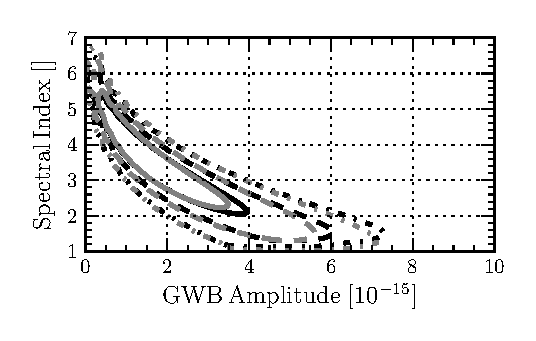
\includegraphics[scale=0.95]{first_compare_1.pdf}
	\label{fig:compareA}}
  \subfigure[]{
  	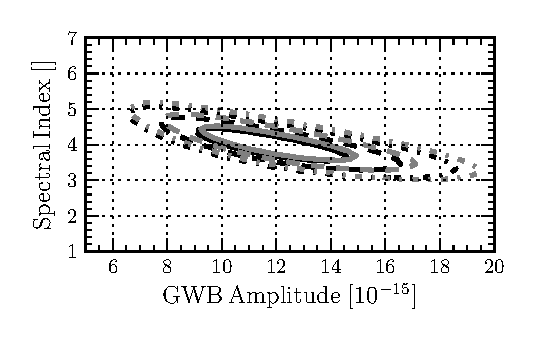
\includegraphics[scale=0.95]{first_compare_2.pdf}
	\label{fig:compareB}}\\
   \end{center}
  \caption{Comparison of full likelihood (gray) of \citet{hlm+09} and the first order likelihood (black). (a): 10 pulsars $A=1\times 10^{-15}$, (b): 10 pulsars $A=1\times 10^{-14}$ }
\label{fig:compare}
\end{figure*}
%%
 In Figure \ref{fig:compareA} we have injected a stochastic GWB with $A=1\times 10^{-15}$ and $\gamma=13/3$. First we notice that the injected value ('$\times$' marker) is well within the 1-sigma credible regions for both likelihood functions. We also see that the confidence contours are nearly identical, with the first order likelihood preferring slightly larger amplitudes and smaller spectral indices. This simulation indicates that the first order likelihood is a very good approximation to the full likelihood when our signal is relatively small, showing no discernible bias and faithfully reproducing nearly identical credible regions. 
 
 In Figure \ref{fig:compareB} we have injected a stochastic GWB with $A=1\times 10^{-14}$ and $\gamma=13/3$. Again, the injected value lies within the 1-sigma credible region, however; now we do notice a difference between two credible regions from the full and first order likelihoods. The first order likelihood is biased towards lower amplitudes and lower spectral indices. In fact we can almost see where the first order approximation begins to break down. Notice that the contours are nearly identical for lower amplitudes and deviate more with increasing amplitude. This behavior is not surprising in that we know that this likelihood is only an unbiased estimator to first order in the amplitude as shown in Section \ref{sec:likelihood}. In fact, it is impressive that this approximation performs this well with only a small bias in the large signal limit (even with timing residuals lower than 100 ns in many pulsars, the signal-to-noise-level of the data simulated here is well above any reasonable estimates for future PTA sensitivities.). This bias will be discussed further in Section \ref{sec:edf}.
 
We now turn to the question of detection. In a Bayesian analysis we would like to compute the odds that there is a GWB present in our data. Not surprisingly, the tool normally used to this end is the Odds ratio of Bayes factor. Consider two models that we will label $M_{1}$ and $M_{2}$, then the Odds ratio is defined as
\be
\mathcal{O}=\mathcal{B}(M_{1},M_{2}|\mathbf{r})\frac{p(M_{1})}{p(M_{2})},
\ee
 where
 \be
 \mathcal{B}(M_{1},M_{2}|\mathbf{r})=\frac{\int d\vec\theta_{1}\,p(\mathbf{r}|\vec\theta_{1},M_{1})p(\vec\theta_{1})}{\int d\vec\theta_{2}\,p(\mathbf{r}|\vec\theta_{2},M_{2})p(\vec\theta_{2})}
 \ee
 is the Bayes factor (i.e the ratio of the marginalized likelihood functions over parameters $\vec\theta_{1}$ and $\vec\theta_{2}$ corresponding to models $M_{1}$ and $M_{2}$ respectively), $\mathbf{r}$ is our data and $p(M_{1})$ and $p(M_{2})$ are the a priori probabilities on models $M_{1}$ and $M_{2}$ respectively. Note that the Bayes factor is the data dependent part of the odds ratio where the a priori probabilities of the models is somewhat subjective, and as such, we will only consider Bayes factors when discussing detection in the this work \footnote{It is possible to use astrophysical information such as the expected level of the stochastic background compared to our noise or the expectation number of single sources to construct the a priori probabilities. Here we will quantify our ignorance by considering equal a priori probabilities of all tested models.}. For our purposes, we would like to compare at least three different models when weighing the odds of a stochastic GWB in our data:
 \begin{enumerate}
 
 \item $M_{\rm gw}$: A power law stochastic GWB with spatial correlations described by the Hellings and Downs coefficients $\zeta_{\alpha\beta}$, amplitude $A_{\rm gw}$ and power spectral index $\gamma_{\rm gw}$, individual power law red noise processes for each pulsar with amplitude $A_{\alpha}$ and power spectral index $\gamma_{\alpha}$ and white noise for each pulsar characterized by an EFAC parameter $\mathcal{F}_{\alpha}$ and EQUAD parameter $\mathcal{Q}_{\alpha}$.
 
 \item $M_{\rm corr}$: A common red noise process among pulsars (as suggested in \cite{sc10}) with no spatial correlations and individual intrinsic red and white components as in model $M_{\rm gw}$.
 
 \item $M_{\rm null}$: Only intrinsic red and white noise processes with no common red or white noise components among pulsars.
 
 \end{enumerate}
 Comparing models $M_{\rm gw}$ and $M_{\rm null}$ will tell us whether or not there is evidence for any common red noise in our data but it will not necessarily tell us that this common noise is due to the stochastic GWB or some other common red noise source. Hence, a large Bayes factor $\mathcal{B}(M_{\rm gw},M_{\rm null}|\mathbf{r})$ is necessary but not sufficient for detection. However, the comparison of models $M_{\rm gw}$ and $M_{\rm corr}$ can really give us information about the nature of the common red noise signal. As the two aforementioned models are identical except for the spatial correlations, a large Bayes factor $\mathcal{B}(M_{\rm gw},M_{\rm corr}|\mathbf{r})$ will give us the odds that there is a common red noise process described spatial correlations  $\zeta_{\alpha\beta}$. Since these \emph{spatial} correlations are the signature of a stochastic GWB, the condition that this   Bayes factor be large is both the necessary and sufficient condition for detection. In fact, this Bayes factor is closely related to signal-to-noise ratios in previous detection schemes \citep{jhl+05,abc+09,ych+11,cce+12} that measure the significance of the cross correlations.
 
This first order likelihood approximation has already been tested on the open and closed \citep{esc12b} IPTA Mock Data Challenge, where all challenges consisted of 130 data points per pulsar with 36 pulsars. For the closed data challenge, we have computed the Bayes factors mentioned in the previous section. In \cite{esc12b} we have shown that we do indeed see very strong evidence for both a common red noise signal and a red noise signal with spatial correlations described by the Hellings and Downs coefficients. However, as we mentioned above, although in this case, the evidence for both models $M_{\rm gw}$ and $M_{\rm corr}$ is very high, as we expect, the Bayes factor $\mathcal{B}(M_{\rm gw},M_{\rm null})$ is much larger than $\mathcal{B}(M_{\rm gw},M_{\rm corr})$.  For this reason, we expect that in analysis of real PTA data we will begin to see strong evidence for common red noise before we are able to see strong evidence for the expected cross correlations. In other words, as we gain more sensitivity, the first two terms in Eq. \ref{eq:foLike} will dominate the likelihood function and the third term will only play a significant role as our sensitivity increases further. A full analysis of this feature along with projected sensitivity curves based on future pulsar timing campaigns and hardware upgrades will be explored in future work.


%While our first-order likelihood method has performed well on the closed MDCs. The open datasets, in particular open MDC1, act as illustrative cases where the first-order approximation breaks down and shows a large bias in parameter estimation. (Show plot or Rutger's results along with ours).

The simulations used in the work have been quite ideal and do not contain any systematic effects such as clock errors which can manifest as a correlated noise source with uniform correlation coefficients (maybe cite Yardley paper), errors in solar system ephemerides (cite something), which can manifest as dipole signals in the residuals, or new physics such as non-gr polarization modes \citep{ljp08,ss12} or massive gravitons \citep{ljp+10} which would change the shape of the Hellings and Downs curve. We have, for the most part, also assumed that the intrinsic pulsar noise can be assumed to be white gaussian noise with no discernible red noise. While previous work suggests that there will be red noise present in many MSPs \citep{sc10}, analyses of the present timing data \citep{vhj+11,delphine,esd+12} suggest that the data is white noise dominated and there is little to no evidence for red noise. However further study of the model selection problem taking in to account the aforementioned effects is crucial to present detection efforts and will be the subject of a future paper.

\subsection{The Empirical Distribution Function}
\label{sec:edf}

Here we will test the consistency and unbiasedness  of our model through injections. Simply put, we wish to show that for $x$\% of realizations, the true injected parameter lies within the inner $x$\% of the marginalized posterior distribution. A similar test was done recently in \cite{vhl12} in \emph{one} dimension through the use of the empirical distribution function (EDF). Here we will review this method and generalize it to two dimensional marginalized posterior distributions. We define the inner high-probability region (HPR) of the two-dimensional marginalized posterior distribution as
\be
\begin{split}
\int_{W}p(\theta_{1},\theta_{2})d\theta_{1}d\theta_{2}&=a\\
W&=\{ \theta_{1},\theta_{2}\in \mathbb{R} : p(\theta_{1},\theta_{2})>L_{a}\},
\label{eq:hpr}
\end{split}
\ee
where $L_{a}$ is some value $>0$ unique to each $a$ that corresponds to a curve of equal probability in the two-dimensional parameter space. In practice we lay down a grid in this two-dimensional parameter space and perform our search over the two parameters of interest (for the stochastic background we search over $A$ and $\gamma$, the dimensionless strain amplitude and power spectral index of the GWB). We then define a set of points $\{A_{i},\gamma_{i}\}\in \mathcal{S}_{a} : p(A_{i},\gamma_{i})>L_{a}$, that is to say we find all points in our grid that correspond to posterior values that lie inside our contour curve $L_{a}$. To determine if the injected values of $\{A_{\rm true},\gamma_{\rm true}\}$ lie within the HPR we simply check to see if the injected values are consistent with the set $\mathcal{S}_{a}$. To do this we first define the complementary set to be $\bar{\mathcal{S}}_{a}$ such that points that are in this set are outside or the HPR. Now we define two chi-squared functions in the parameter space
\begin{align}
\chi_{a}(A_{i},\gamma_{i})^{2}&=\left(\frac{A_{i}-A_{\rm true}}{A_{\rm true}}\right)^{2}+\left(\frac{\gamma_{i}-\gamma_{\rm true}}{\gamma_{\rm true}}\right)^{2}\\
\bar{\chi}_{a}(A_{j},\gamma_{j})^{2}&=\left(\frac{A_{j}-A_{\rm true}}{A_{\rm true}}\right)^{2}+\left(\frac{\gamma_{j}-\gamma_{\rm true}}{\gamma_{\rm true}}\right)^{2},
\end{align}
where $\{A_{i},\gamma_{i}\}$ and $\{A_{j},\gamma_{j}\}$ are elements of the sets $\mathcal{S}_{a}$ and $\bar{\mathcal{S}}_{a}$, respectively. Finally, we define the empirical distribution function (EDF) as
\be
F_{k}(a)=\frac{1}{k}\sum_{n=1}^{k}\Theta(\min \bar{\chi}_{a}^{2}-\min \chi_{a}^{2}),
\ee
where $\Theta(x)$ is the Heaviside function. The term inside the sum indicates an event when the injected values are ``closer'' (in the chi-squared sense) to one of the elements of $\mathcal{S}_{a}$ than to any of the elements of $\bar{\mathcal{S}}_{a}$, therefore we can say that the values $\{A_{\rm true},\gamma_{\rm true}\}$ join the set $\mathcal{S}_{a}$ and lie within the HPR defined in Eq. \ref{eq:hpr}. Now that we have defined our EDF, the rest of the analysis mimics \cite{vhl12}.

For this analysis we simulated 1000 datasets for 6 different scenarios. In all cases we chose the white noise level to be 100 ns while we chose GWB amplitudes of $1\times 10^{-15}$, $2\times 10^{-15}$, and $3\times 10^{-15}$ for PTAs with both 10 and 15 pulsars with a 5 year baseline. Figure \ref{fig:combined_edf} shows the EDF for the six models outlined above. 
%%
\begin{figure}[!h]
  \begin{center}
  %\showthe\columnwidth
	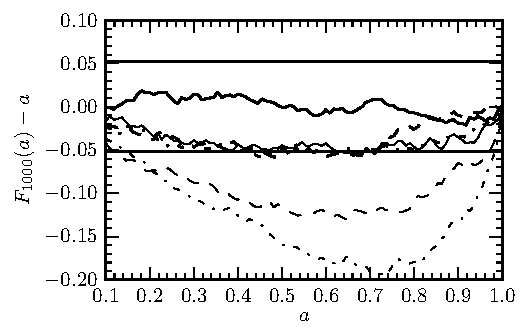
\includegraphics[width=\columnwidth]{edf_all.pdf}
  \end{center}
  \caption{Empirical distribution function for 6 scenarios. The thick lines denote a 10 pulsar PTA and the thin lines denote a 15 pulsar PTA and the solid, dashed and dotted lines denote injected stochastic GWB amplitudes of  $1\times 10^{-15}$, $2\times 10^{-15}$, and $3\times 10^{-15}$, respectively. The solid lines at $\pm 0.052$ represent the value at which we should reject the null-hypothesis that our analysis method is consistent and unbiased. }
\label{fig:combined_edf}
\end{figure}
%%
The thick lines denote a 10 pulsar PTA and the thin lines denote a 15 pulsar PTA and the solid, dashed and dotted lines denote injected stochastic GWB amplitudes of  $1\times 10^{-15}$, $2\times 10^{-15}$, and $3\times 10^{-15}$, respectively. The solid lines at $\pm 0.052$ represent the value at which we should reject the null-hypothesis that our analysis method is consistent and unbiased. Firstly, we note that for both the 10 and 15 pulsar PTA, our analysis method is consistent for an injected amplitude of $A=1\times 10^{15}$ (maybe put some reference to how large the signal is on average compared to white noise). We obtain similar results in the 10 pulsar case for amplitudes of $A=2\times 10^{-15}$ and $A=3\times 10^{-15}$. Here we do see that our method is indeed slightly biased for these larger amplitudes but the degree of bias is almost negligible. However, for these same amplitudes in the 15 pulsar case there is a significant bias. Even though there is a bias present in these scenarios, the EDF does not give information about how this bias presents itself in the two dimensional parameter space. 
%%
\begin{figure*}[!t]
  \begin{center}
  %\showthe\columnwidth
	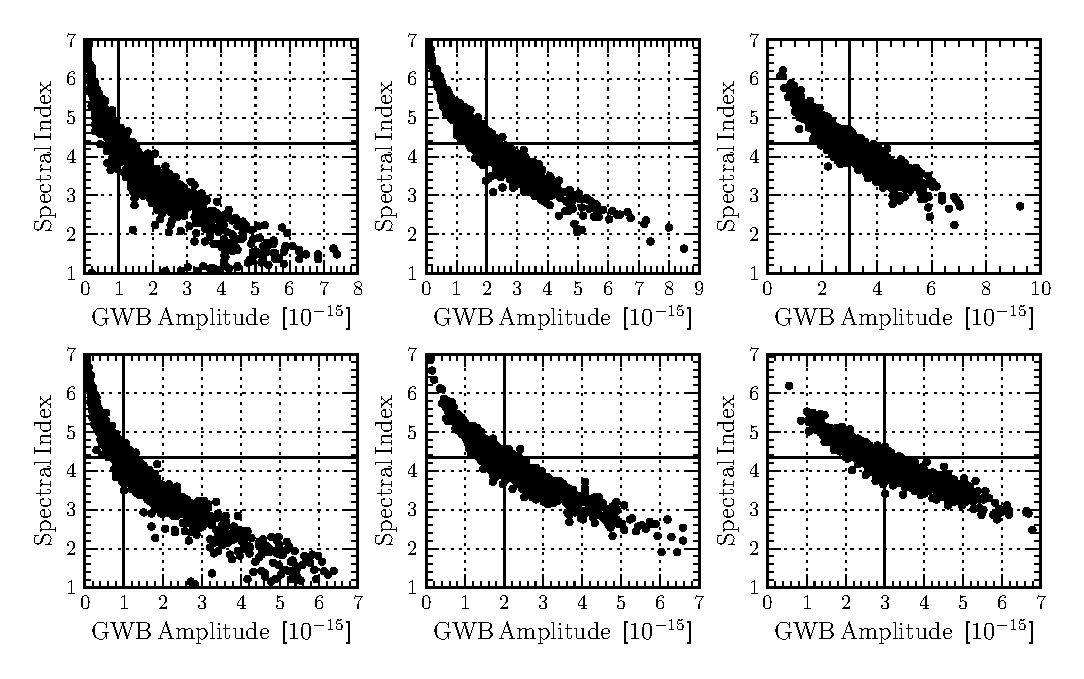
\includegraphics[scale=1.0]{EDF_scatter.pdf}
  \end{center}
  \caption{Here we show the scatter of the maximum likelihood values of the GWB amplitude and spectral index from the Monte-Carlo simulations. From left to right the injected amplitudes are $1\times 10^{-15}$, $2\times 10^{-15}$, and $3\times 10^{-15}$ with spectral index $13/3$ for a 10 pulsar PTA (top row) and 15 pulsar PTA (bottom row). We can see that nearly all of these distributions display minimal bias. }
\label{fig:edf_scatter}
\end{figure*}
%%
In Figure \ref{fig:edf_scatter} we show the two-dimensional scatter plot of the maximum likelihood parameters from our Monte-Carlo simulations. It is clear that the bias in our two-dimensional parameter space of interest is \emph{practically} very small. In fact the means of the distributions for $A$ and $\gamma$ for the 10 pulsar case are $(1.6,2.25,3.14)\times 10^{-15}$ and $(4.17,4.24,4.23)$, respectively and for the 15 pulsar case we obtain $(1.56,2.29,3.22)\times 10^{-15}$ and $(4.11,4.12,4.13)$, respectively. In the first row of Figure \ref{fig:edf_scatter} we show the 10 pulsar case with increasing GWB amplitude and the second row we show the same for the 15 pulsar case. In the cases where there is a bias present, the likelihood function prefers slightly lower spectral indices and slightly larger amplitudes. However, from our experience with the MDC this bias can also present itself by preferring a slightly higher spectral index and lower amplitude.   It should  be noted that even the smallest of the amplitudes tested here are near the upper range of  the expected level of the stochastic GWB \citep{s13} and that the white noise rms of the pulsars is slightly unrealistic in our current PTA regime. In fact we expect to have maybe five or six pulsar that time at or below the 100 ns level while we have many others that have much larger white noise rms. Thus we can conclude that even though our likelihood is somewhat biased at larger amplitudes (as is expected), for \emph{realistic} astrophysically likely stochastic GWBs this method is effectively consistent and unbiased. In fact, in terms of setting upper limits on the stochastic GWB amplitude (cite), this method is practically identical to using the full likelihood, while much more computationally efficient.


\section{Discussion and Conclusions}
\label{sec:conclusions}
Here will will briefly discuss future prospects of conducting a simultaneous search for continuous GWs and the stochastic GWB. We will also compare our work to other recent efforts to speed up PTA GW data analysis and discuss the importance of our first-order likelihood method.

\subsection{Simultaneous Detection of Continuous GWs and a Stochastic GWB}

One very important feature of the first order likelihood method is that it can also be applied to searches for continuous GWs. This will allow us to simultaneously search for a correlated stochastic background and resolve individual sources that are bright enough to stand out above such a background. In standard continuous GW searches using PTAs \citep{bs12,esc12,pbs+12} the assumption is made that any detectable single source will be bright enough such that the noise (e.g stochastic GWB) can be approximated as a gaussian process that is uncorrelated among pulsars. However, recent work \citep{rwh+12} has shown that we are likely to see a few single sources per frequency bin that will stand out from the typical isotropic stochastic background, thus in order to resolve the weakest of these it is crucial to simultaneously search for a correlated stochastic background as well as the continuous source. We can then write down a combined likelihood function assuming a deterministic source of functional form $\mathbf{s}(\vec\lambda)$
\be
p(\mathbf{r}|\vec{\theta},\vec{\lambda})=\frac{1}{\sqrt{\det2\pi\boldsymbol{\Sigma}}}\exp\lp -\frac{1}{2}(\mathbf{r}-\mathbf{s})^{T}
\boldsymbol{\Sigma}^{-1}(\mathbf{r}-\mathbf{s}) \rp,
\label{eq:singleFull}
\ee
where our noise (including the stochastic background) parameters are $\vec\theta$ and our single source parameters are $\vec\lambda$. Using our first order likelihood approach we can approximate Eq. \ref{eq:singleFull} as
\begin{widetext}
\be
\begin{split}
\ln\,p(\mathbf{r}|\vec{\theta},\vec{\lambda}) &=\approx-\frac{1}{2}\left[ \Tr\ln \mathbf{P} +(\mathbf{r}-\mathbf{s})^{T}\mathbf{P}^{-1}(\mathbf{r}-\mathbf{s})-(\mathbf{r}-\mathbf{s})^{T}\mathbf{P}^{-1}\mathbf{S}_{c}\mathbf{P}^{-1}(\mathbf{r}-\mathbf{s})  \right]\\
&=-\frac{1}{2}\sum_{\alpha=1}^M \left[\Tr\ln P_{\alpha} +(r_{\alpha}-s_{\alpha})^TP_{\alpha}^{-1}(r_{\alpha}-s_{\alpha}) -\sum_{\beta\ne\alpha}^M(r_{\alpha}-s_{\alpha})^T P_{\alpha}^{-1}S_{\alpha\beta}P_{\beta}^{-1}(r_{\beta}-s_{\beta})\right].
\end{split}
\ee
\end{widetext}
As in the stochastic background case, this again will speed up computations because we only have to invert the \emph{individual} auto-covariance matrices as opposed to the \emph{full} data covariance matrix. Although there have been proposed methods to speed up the computation of the stochastic likelihood function of Eq. \ref {eq:liker} \citep{vh12}, this is not applicable to continuous sources because it relies on essentially applying a low pass filter to the data. However, since we expect continuous sources across the entire frequency band (with higher frequency sources possibly standing out above the background) we must keep all frequency information. Therefore our first order likelihood approximation is a viable option when looking to significantly speed up computation time while losing minimal information about potential GW signals.

As always, to claim a detection we must do some sort of model comparison, be it a Neyman-Pearson test for Frequentist statistics or an odds ratio or Bayes factor for Bayesian statistics. For example if we want to assess the likelihood of that a continuous GW is in our data we want to compute the following Bayes factor
\be
\mathcal{B}=\frac{\mathcal{Z}_{\rm CW}}{\mathcal{Z}_{\rm noise}}=\frac{\int\int d\vec{\lambda}d\vec{\theta}p(\mathbf{r}|\vec\theta,\vec\lambda)p(\vec{\lambda})p(\vec{\theta})}{\int d\vec{\theta}p(\mathbf{r}|\vec\theta)p(\vec{\theta})},
\ee
where $\mathcal{Z}_{\rm CW}$ and $\mathcal{Z}_{\rm noise}$ are the evidence for the gravitational CW and noise models, respectively. However, notice that $\vec\theta$ depends on our stochastic GWB parameters as we treat all stochastic processes as ``noise'' in this analysis. If we do not include the GWB parameters in the model then we could mistake a low frequency GWB for a single continuous source, thus including the GWB stochastic background in both models is crucial to detection and eventually characterization of a single GW source. We should also mention that the biases mentioned in section \ref{sec:edf} are not as important if we simply wish to let the noise parameters vary along with the single source parameters since these noise parameters will be marginalized over in the end. An exploration of these combined searches will be the subject of a future paper. 

\subsection{Comparison with Other Work}

Recently there have been three studies devoted to making the analysis of PTA data more computationally efficient. First, \citet{vh12} have developed a method dubbed Acceleration By Compression (ABC) to speed up this analysis. The main point of this work is to write the data in a compressed basis, keeping the minimum number of basis vectors to maximize the ability to characterize a correlated red signal. This work also makes use of an interpolation scheme to compute the covariance matrix which further improves the efficiency of the algorithm at the cost of large memory usage. This method has proved to be very efficient and accurate in setting upper limits on the stochastic GWB and characterizing injected signals. However, since this method relies on a reduced basis that essentially ``throws away'' high frequency information it is impossible to obtain a reliable Bayes Factor when comparing models that allow for varying white noise components. Since our first-order likelihood function makes use of all the information in the data we can indeed compute reliable Bayes factors and make confident statements about detection. 

Most recently there have been two analyses of the IPTA MDC that aim to make the PTA data analysis more efficient. First, \citet{Lentati:2012xb} have developed a novel model-independent method for the estimation of the spectral properties of an isotropic stochastic GWB. This method uses a frequency domain approach and is extremely efficient and results in computational speedups of two to three orders of magnitude over the full likelihood implementation. It has also been extensively tested on the MDC datasets and has proved to be very accurate in characterizing the stochastic GWB. Our first order likelihood method is indeed complementary to this work as it provides a way to efficiently evaluate the likelihood function in a full time domain analysis which will be vital for cross-checks for real-life detection candidates.

Finally, \citet{Taylor:2012vx} have implemented the full VHML likelihood function and have made it more efficient through the use of optimized linear algebra libraries with multithreading and parallelization resulting in significant speedups in the likelihood evaluation. However, all of these methods could just as well be applied to the first-order likelihood which would still be more efficient than the full likelihood by a factor proportional to the number of pulsars in the array. 

This work and recent work have shown that there has indeed been significant progress on making the likelihood evaluation more efficient for pulsar timing arrays. All of these methods are complementary and will provide important cross checks for future stochastic GWB detection candidates.

\subsection{Summary}

In this paper we have introduced a novel way to speed up the computation of the likelihood function for PTAs when searching for a stochastic GWB. This was accomplished by expanding the likelihood function to first order in the Hellings and Downs correlation coefficients expected for a stochastic GWB leading to a computational speedup on the order of the square of the number of pulsars in the PTA. For typical PTAs this results in a speed-up of a few hundred to about a thousand. We have briefly discussed the implementation of this technique on the first IPTA Mock Data Challenge and showed that this algorithm performs well in extracting the injected GWB parameters and making a significant detection through various Bayes factors. Though this is indeed an approximation to the full likelihood function we have shown through extensive simulations that the bias introduced in the estimation of GWB parameters is minimal and negligible in many cases. This was accomplished through an analytical computation of the expectation value of the maximum likelihood, direct comparisons of the full and first-order likelihood functions on simulated data sets and through a statistical Monte-Carlo approach based on the Empirical Distribution Function. Although this work has focused solely on the detection and characterization of a stochastic GWB, this likelihood function can also be used to estimate the intrinsic red and white noise parameters of individual pulsars simultaneously with the GWB parameters. 

\acknowledgements
We would like to thank the members of the NANOGrav detection working group for their comments and support, especially Paul Demorest and Joe Romano. We would also like to thank Jolien Creighton for useful conversations. This work was partially funded by the NSF through CAREER award number 0955929, PIRE award number 0968126, and award number 0970074.

\appendix

\section{Relationship to VHML likelihood}
\label{app:likelihood}
Making use of Eq. \ref{eq:resids}, the likelihood function for  the noise can be written as
\be
\begin{split}
p(\mathbf{n}|\vec\theta)=p(\mathbf{r}|\vec\theta,\delta\boldsymbol{\xi}_{\rm best})=\frac{1}{\sqrt{\det(2 \pi \boldsymbol{\Sigma}_n)}}
\times\exp\lp-\frac{1}{2}(\mathbf{r}-\mathbf{M}\delta\boldsymbol{\xi}_{\rm best})^T\boldsymbol{\Sigma}_n^{-1}(\mathbf{r}-\mathbf{M}\delta\boldsymbol{\xi}_{\rm best})\rp.
\end{split}
\ee
This can be thought of as a \emph{conditional} pdf, where the values of $\delta\boldsymbol{\xi}_{\rm best}$ are fixed.  In \cite{vhl12} it was shown that the marginalized likelihood can be written as
\be
\begin{split}
p(\mathbf{r}|\vec\theta)=\int d\delta\boldsymbol{\xi}\,p(\mathbf{r}|\vec\theta,\delta\boldsymbol{\xi})
=\frac{\exp\left[ -\frac{1}{2}\mathbf{r}^{T}\mathbf{G}^{T}\lp \mathbf{G}^{T}\boldsymbol{\Sigma}_{n}\mathbf{G} \rp^{-1}\mathbf{G}^{T}\mathbf{r} \right]}{\sqrt{\det 2\pi\mathbf{G}^{T}\boldsymbol{\Sigma}_{n}\mathbf{G}}},
\end{split}
\ee
where $\mathbf{G}$ is the matrix constructed from the final $(N-N_{\rm fit})$ columns of the matrix $\mathbf{U}$ in the singular value decomposition of the design matrix, $\mathbf{M}=\mathbf{U}\mathbf{S}\mathbf{V}^{T}$.

We will now explore the $G$ matrix and the $R$ matrix obtained from the marginalized and conditional pdfs, respectively. As mentioned above, $R$ can be thought of as an oblique projection operator that projects the pre-fit residuals into the post-fit residual space, whereas $G^{T}$ can be thought of a projection operator that projects our data onto the null space of $M$, that is, it projects the data into a subspace orthogonal to the timing model fit. Since $R$ is not generally symmetric and therefore is an oblique projection operator, it does not have such a simple mathematical interpretation. However, we can recast our problem in terms of ``weighted'' residuals then we have the following transformations: $r\rightarrow Wr$, $M\rightarrow WM$, and $R\rightarrow W^{-1}RW$, where $W$ is the weighting matrix defined above. In this case minimizing the chi-squared becomes and unweighted least squares problem and we obtain the exact same estimates of $\delta\boldsymbol{\xi}_{\rm best}$ and  likelihood function as before. In this case $R$ is symmetric and can be thought of as an orthogonal projection operator that projects our weighted data onto the null space of the weighted timing model ($WM$). However, in order to compute the likelihood we still have to invert the covariance matrix $\Sigma_{r}=R\Sigma_{n}R^{T}$ which is singular. To do this we rely on the pseudo-inverse. The pseudo-inverse of $\Sigma_{r}$ is easiest defined in terms of its eigen-decomposition $\Sigma_{r}=EDE^{T}$, with $E$ the matrix of eigenvectors of $\Sigma_{r}$, and $D$ the diagonal matrix with $D_{ii}=\lambda_{i}$ the eigenvalues of $\Sigma_{r}$. It so happens that for a symmetric positive semi-definite matrices like these, the eigen-decomposition is also the singular value decomposition (SVD). The pseudo-inverse of $\Sigma_{r}$ is then
\be
\overline{\Sigma_{r}^{-1}}=E\overline{D^{-1}}D^{T},
\ee  
where the overbar indicates that we are taking a pseudo-inverse and $\overline{D^{-1}}_{ii}=1/\lambda_{i}$ for $\lambda>0$ and $\overline{D^{-1}}_{ii}=0$ otherwise. Note that when all the error bars are the same (i.e. $W=\sigma^{-1}\mathbb{I}$ with $\sigma$ constant), the matrix $G^{T}\Sigma_{n}G$ has the same eigenvalues as the non-singular part of $R\Sigma_{n}R^{T}$ and we have
\be
\overline{(R\Sigma_{n}R^{T})^{-1}}=G(G^{T}\Sigma_{n}G)^{-1}G^{T}.
\ee
Thus we have obtained a very interesting result that in the case of uniform uncertainties, the conditional pdf making use of  a pseudo-inverse is equivalent to the marginalized pdf making use of the projection matrix $G^{T}$. However, in general this is not true and the two methods are indeed different. Although, in many cases the uncertainties are similar on a majority of the TOAs, thus the two methods will not differ much in practice.






\bibliographystyle{apj}
\bibliography{apjjabb,bib}



\end{document}
